%%%%%%%%%%%%%%%%%%%%%%%%%%%%%%%%%%%%%%%%%%%%%%%%%%%%%%%%%%%%%%%%%%%%%%%%%%%%%%%%%%%%%%%%%%%%%%%
%                                        SEGMENTATION                                         %
%%%%%%%%%%%%%%%%%%%%%%%%%%%%%%%%%%%%%%%%%%%%%%%%%%%%%%%%%%%%%%%%%%%%%%%%%%%%%%%%%%%%%%%%%%%%%%%
\chapter{Deformable Shape Models using Deep Learning}
\label{chap:seg}

\begin{chapabstract}
 Coucou
\end{chapabstract}

\vspace{1cm}

{   
    \setstretch{1.0}
    \minitoc
}

\newpage

%%%%%%%%%%%%%%%%%%%%%%%%%%%%%%%%%%%%%%%%%%%%%%%%%%%%%%%%%%%%%%%%%%%%%%%%%%%%%%%%%%%%%%%%%%%%%%%
\section{Template Models}

An approach to the segmentation of medical images is to use a previously acquired template and deform it to match the image to segment. Formally, given a template $\phi_0$ and an image $I$, we are interested in obtaining the segmentation mask $\phi$ by finding the deformation fields $\psi$ to be applied to the image:

\begin{equation}
    \phi = \phi_0 \cdot \psi \left( I \right)
\end{equation}

\subsection{Constructing the template}

There are various strategies to construct the template. One can select the template as the image most similar to the one to segment in an existing database (\textcite{commowick2007MICCAI}) or build a mean template by using multiple images (\textcite{joshi2004}).

Another strategy is to use multiple templates, which increases the robustness of the methods (\textcite{heckemann2006}) and then fuse the predictions (\textcite{warfield2004}). 

A review of the existing methods of template construction can be found in~\textcite{cabezas2011}.

\subsection{Finding the deformation fields}

Many methods such as \textit{Active Shape Models} (\textcite{cootes1995}), \textit{Active Appearance Models} (\textcite{cootes1998ECCV}) or \textit{Implicit Template Deformation} (\textcite{mory2012MICCAI}) have been proposed before. As this thesis focuses on deep learning, they are out-of-scope. We refer the interested reader to~\textcite{heimann2009} for a review of those methods.

To the best of our knowledge, deep learning has not yet been used in the context of template models. It has however been used in the context of registration, i.e. the spatial alignment of two medical images.

Convolutional neural networks have been used to regress the parameters of the registration transform from the input images (\textcite{miao2016},~\textcite{yang2016}).

Another approach is to estimate a similarity measure from a neural network to be used in an iterative optimization strategy (\textcite{wu2013MICCAI},~\textcite{cheng2015},~\textcite{simonovosky2016MICCAI}).

Recently, method using GANs (\textcite{goodfellow2014}) have been proposed.  

[TODO describe GANs approaches]

An Unsupervised Learning Model for Deformable Medical Image Registration (voxelmorph)

Adversarial Similarity Network for Evaluating Image Alignment in Deep Learning Based Registration

%%%%%%%%%%%%%%%%%%%%%%%%%%%%%%%%%%%%%%%%%%%%%%%%%%%%%%%%%%%%%%%%%%%%%%%%%%%%%%%%%%%%%%%%%%%%%%%
\section{Kidney Segmentation in 3D Ultrasound}

The problem addressed is the same as in Section~\ref{sec:kidney}: kidney capsule segmentation in 3D ultrasound data from potentially ill children. The difference is that we are not in a transfer learning setting and we have access to both adults and children images simultaneously.

The contribution of this work is in the novel model-based segmentation method presented in Section~\ref{sec:deformable_dl}. We compare performance of the method to a baseline 3D U-Net and discuss their results in Section~\ref{sec:seg_result}.

%%%%%%%%%%%%%%%%%%%%%%%%%%%%%%%%%%
%\subsection{Dataset}

\begin{figure}[htb]
        \begin{subfigure}[b]{0.245\textwidth}
                \centering
                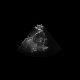
\includegraphics[width=\linewidth]{img_seg/30_post}
        \end{subfigure}%
        \hspace{1px}
        \begin{subfigure}[b]{0.245\textwidth}
                \centering
                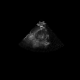
\includegraphics[width=\linewidth]{img_seg/32_post}
        \end{subfigure}%
        \begin{subfigure}[b]{0.245\textwidth}
                \centering
                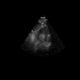
\includegraphics[width=\linewidth]{img_seg/33_post}
        \end{subfigure}%
        \begin{subfigure}[b]{0.245\textwidth}
                \centering
                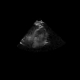
\includegraphics[width=\linewidth]{img_seg/37_post}
        \end{subfigure}
        
        \begin{subfigure}[b]{0.245\textwidth}
                \centering
                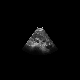
\includegraphics[width=\linewidth]{img_seg/70_post}
        \end{subfigure}%
        \hspace{1px}
        \begin{subfigure}[b]{0.245\textwidth}
                \centering
                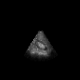
\includegraphics[width=\linewidth]{img_seg/71_post}
        \end{subfigure}%
        \begin{subfigure}[b]{0.245\textwidth}
                \centering
                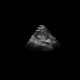
\includegraphics[width=\linewidth]{img_seg/72_post}
        \end{subfigure}%
        \begin{subfigure}[b]{0.245\textwidth}
                \centering
                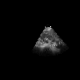
\includegraphics[width=\linewidth]{img_seg/75_post}
        \end{subfigure}
        
        \begin{subfigure}[b]{0.245\textwidth}
                \centering
                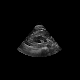
\includegraphics[width=\linewidth]{img_seg/280_post}
        \end{subfigure}%
        \hspace{1px}
        \begin{subfigure}[b]{0.245\textwidth}
                \centering
                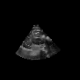
\includegraphics[width=\linewidth]{img_seg/282_post}
        \end{subfigure}%
        \begin{subfigure}[b]{0.245\textwidth}
                \centering
                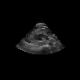
\includegraphics[width=\linewidth]{img_seg/286_post}
        \end{subfigure}%
        \begin{subfigure}[b]{0.245\textwidth}
                \centering
                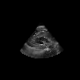
\includegraphics[width=\linewidth]{img_seg/288_post}
        \end{subfigure}
        \caption{Original images after pre-processing (left column) and augmented images (other three columns).}
        \label{fig:data_aug}
\end{figure}

The dataset stays identical as in Section~\ref{ssec:data}, as well as the pre-processing. We have 503 healthy adults images and 64 children. The images have been down-sampled to a resolution of $4 \times 4 \times 4$ mm$^3$, and centered in a $80 \times 80 \times 80$ voxels cube. 

\begin{table}[htb]
	\centering
	\begin{tabular}{|l|c|c|}
	    \hline
                        & Mean & Standard deviation \\
        \hline
         Gaussian noise & $0$ & $5$ \\
         Translation & $0$ & $3$ \\
         Rotation & $0$ & $0.05$ \\
         Scaling & $1$ & $0.05$ \\
        \hline
    \end{tabular}
	\caption{Data augmentation used for the kidney dataset. The parameters for each type of augmentation are drawn from a normal distribution with the mean and standard deviation specified.}
	\label{table:data_aug}
\end{table}

Unlike previously, we use data augmentation. Due to the already high cost of training on this dataset, each image is augmented 10 times before training. The augmentation includes adding Gaussian noise, as well as translation, rotation and scaling of the image (and the segmentation). The range of each type of augmentation is shown in Table~\ref{table:data_aug}. Some augmented images are shown in Figure~\ref{fig:data_aug} alongside their original image.

%%%%%%%%%%%%%%%%%%%%%%%%%%%%%%%%%%%%%%%%%%%%%%%%%%%%%%%%%%%%%%%%%%%%%%%%%%%%%%%%%%%%%%%%%%%%%%%
\section{Deformable shape models and deep learning}
\label{sec:deformable_dl}

We propose in this section to train a neural network to predict the deformation required for a shape model to match a segmentation target on a specific image. There are two components: predicting a geometric transformation and predicting the deformation field.

\begin{figure}[htbp]
	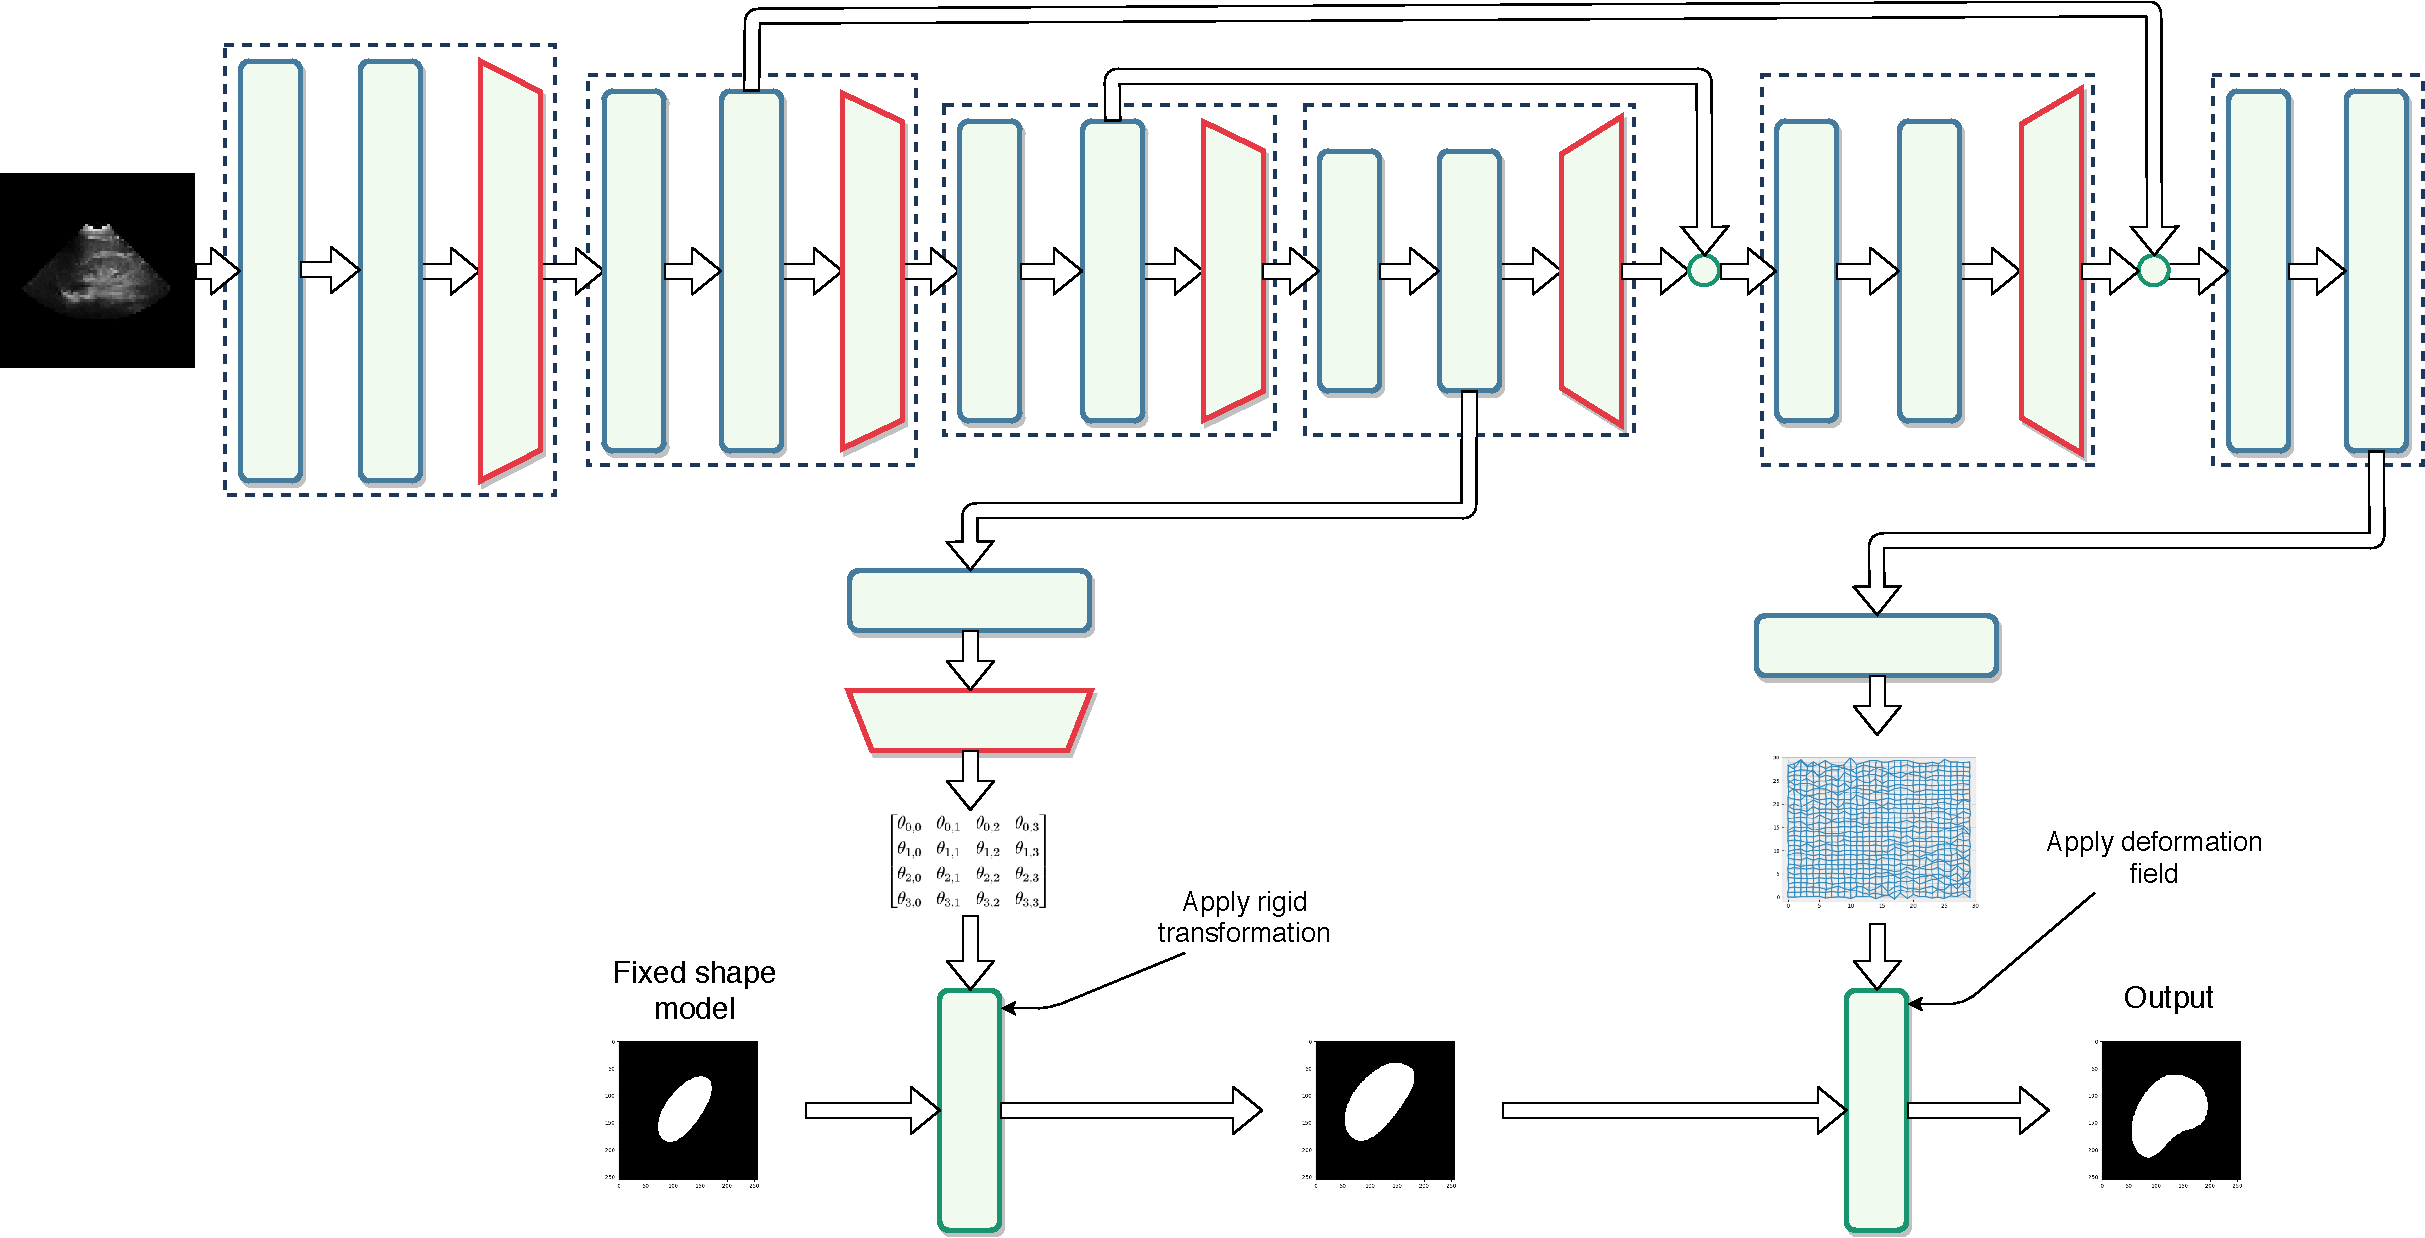
\includegraphics[width=\textwidth]{img_seg/deformation_network}
    \caption{Segmentation network that predicts a geometric transformation and a deformation field to deform a shape model.}
    \label{fig:deform_network}
\end{figure}

Figure~\ref{fig:deform_network} presents the process. The network predict a geometric transformation $G$ and a deformation field $\psi$ from the image, which are applied to a template $\phi_0$. The deformed template then corresponds to the correct segmentation for the image.

\begin{equation}
    \phi = \phi_0 \cdot G \cdot \ \psi
\end{equation}

In our case, the template is the ground truth segmentation from an image not included in the training, validation or test sets.

The next sections explains how to predict and apply the transformation and the deformation field.

\subsection{Predicting a geometric transformation}

A geometric transformation for 3D images is represented by a $4 \times 4$ matrix, meaning a total of 16 parameters that can be predicted. Directly predicting those parameters remove control on the kind of transformation that are predicted. In our case, we chose to predict instead translation, rotation and scaling parameters. 

Three parameters are predicted for the translation on each axis, giving the following translation matrix $T$:
\begin{equation*}
    T = 
    \begin{bmatrix}
        1 & 0 & 0 & t_x \\
        0 & 1 & 0 & t_y \\
        0 & 0 & 1 & t_z \\ 
        0 & 0 & 0 & 1
    \end{bmatrix}
\end{equation*}

The scaling matrix $S$ is built from three more parameters:
\begin{equation*}
    S = 
    \begin{bmatrix}
        s_x & 0 & 0 & 0 \\
        0 & s_y & 0 & 0 \\
        0 & 0 & s_z & 0 \\ 
        0 & 0 & 0 & 1
    \end{bmatrix}
\end{equation*}

Finally, we have one rotation matrix in each direction ($R_x$, $R_y$ and $R_z$) built from one parameter each:
\begin{equation*}
    R_x = 
    \begin{bmatrix}
        1 & 0 & 0 & 0 \\
        0 & \cos{r_x} & -\sin{r_x} & 0 \\
        0 & \sin{r_x} & \cos{r_x} & 0 \\ 
        0 & 0 & 0 & 1
    \end{bmatrix}
\end{equation*}
\begin{equation*}
    R_y = 
    \begin{bmatrix}
        \cos{r_y} & 0 & - \sin{r_y} & 0 \\
        0 & 1 & 0 & 0 \\
        \sin{r_y} & 0 & \cos{r_y} & 0 \\ 
        0 & 0 & 0 & 1
    \end{bmatrix}
    \mkern20mu
    R_z = 
    \begin{bmatrix}
        \cos{r_z} & -\sin{r_z} & 0 & 0 \\
        \sin{r_z} & \cos{r_z} & 0 & 0 \\
        0 & 0 & 1 & 0 \\ 
        0 & 0 & 0 & 1
    \end{bmatrix}
\end{equation*}

We also need to center the image around zero before applying the rotations, which requires no parameters except knowing the center of the image:
\begin{equation*}
    C_+ = 
    \begin{bmatrix}
        1 & 0 & 0 & c_x \\
        0 & 0 & 0 & c_y \\
        0 & 0 & 0 & c_z \\ 
        0 & 0 & 0 & 1
    \end{bmatrix}
    \mkern20mu
    C_- = 
    \begin{bmatrix}
        1 & 0 & 0 & -c_x \\
        0 & 0 & 0 & -c_y \\
        0 & 0 & 0 & -c_z \\ 
        0 & 0 & 0 & 1
    \end{bmatrix}
\end{equation*}

From these matrices, the geometric transformation $G$ applied to the shape model is the following:
\begin{equation}
    G = T \cdot C_+ \cdot R_z \cdot R_y \cdot R_x \cdot S \cdot C_-
\end{equation}

The prediction of the 9 required parameters is done by a convolutional layer with 9 $1 \times 1 \times 1$ filters, followed by an average pooling layer of the size of the feature maps. 

\subsection{Predicting a deformation field}

The deformation field are predicted from a convolutional layer with 3 $3 \times 3 \times 3$ filters, one filter per dimension. Each field is then smoothed with a $3 \times 3 \times 3$ mean filter, before being resized to the shape model size with a tri-linear interpolation. This resizing step allows predicting deformation fields at a lower resolution than the shape model, saving time and parameters to learn.

We added an $L_2$ penalty term to the deformation fields $\psi$ in the loss function:
\begin{equation}
    P = \lambda \sum_x \left( \psi - Id \right)(x)^2
\end{equation}
$Id$ is the identity matrix and $\lambda$ is the strength of this term, chosen as $10^{-3}$. The goal of this penalty term is to constrain the size of the deformation fields.

% \subsection{Distance map and loss}

% - Distance map and appropriate loss

%%%%%%%%%%%%%%%%%%%%%%%%%%%%%%%%%%%%%%%%%%%%%%%%%%%%%%%%%%%%%%%%%%%%%%%%%%%%%%%%%%%%%%%%%%%%%%%
\section{Results and Discussion}
\label{sec:seg_result}

\begin{table}[htbp]
	\centering
\begin{tabular}{|l|c|c|c|c|}
	\hline
    Method & Dice Adults & Dice Children \\
	\hline
    3D U-Net & $\bm{0.89}$ & $\bm{0.82}$ \\
    Deformation & $0.85$ & $0.75$ \\
    Geometric transfo + Deformation & $0.88$ & $\bm{0.82}$ \\
    Geometric transfo + Deformation + $L_2$ penalty & ??? & ??? \\
    \hline
\end{tabular}
	\vspace{2mm}
	\caption{Performance of the baseline and the shape model methods.}
    \label{table:seg_results}
\end{table}

For all the models the training is done jointly on adults and children with oversampling of the children to balance the populations. Each model was trained on only one seed due to the high cost of training (around five days per model). The performance of each model is reported in Table~\ref{table:seg_results}.

The baseline for our comparison is the 3D U-Net (\textcite{cicek2016MICCAI}) described in Section~\ref{ssec:unet}. Its performance is therefore comparable to the one reported in Section~\ref{sec:kidney_res}, the only difference being the use of data augmentation. The performance goes from $0.81$ for the adults and $0.74$ for the children to $0.89$ and $0.82$, an important increase of $0.08$ for both populations. 

Training a model predicting only deformation fields without the geometric transformation is not enough to beat the baseline, though it does show that the idea works. When adding the geometric transformation, the results become very close to the baseline. The geometric transformation is beneficial in particular for the children. This is likely due to the fact that the template model is an adult kidney, requiring the network to learn how to shrink it when segmenting children images. The geometric transformation provides an easy way to learn this shrinking with the three scaling parameters.

[TODO penalty results]

% \begin{figure}[htbp]
%   \begin{subfigure}[b]{0.5\linewidth}
%     \centering
%     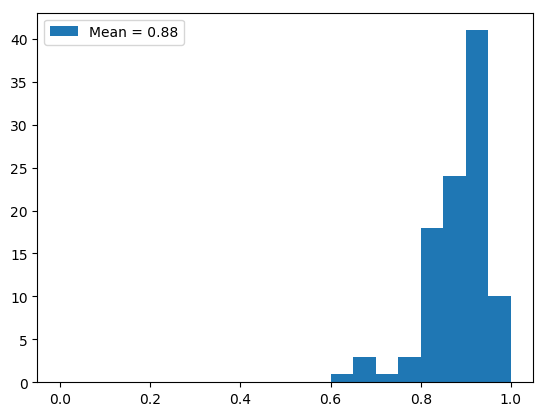
\includegraphics[width=0.95\linewidth]{img_seg/dice_hist_adults} 
%   \end{subfigure}%% 
%   \begin{subfigure}[b]{0.5\linewidth}
%     \centering
%     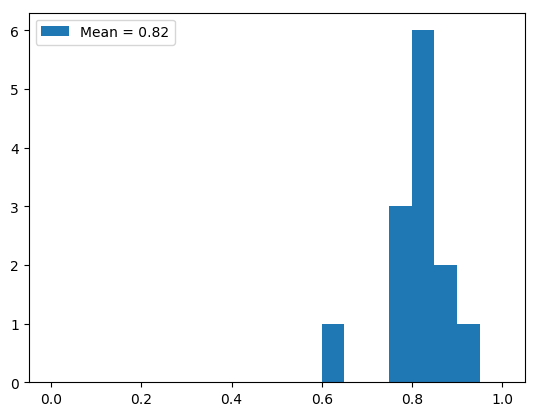
\includegraphics[width=0.95\linewidth]{img_seg/dice_hist_children} 
%   \end{subfigure} 
%   \caption{Histograms of Dice coefficient for the model with geometric transformation and deformation fields. Left: Dice coefficient on adults, right: Dice coefficient on children.}
%   \label{fig:seg_hist}
% \end{figure}

\begin{figure}[htbp]
    \centering
	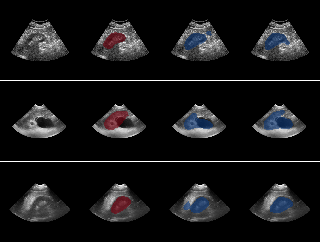
\includegraphics[width=\textwidth]{img_seg/unet_vs_deform}
    \caption{Comparing 3D U-Net results and deformation fields results. From left to right: image, ground truth, U-Net segmentation, deformation fields segmentation.}
    \label{fig:unet_vs_deform}
\end{figure}

Even though the performance of our method is similar to the baseline, using the template model results in segmentation anatomically correct. There are no patches of disconnected voxels classified as kidney or unlikely shapes. In Figure~\ref{fig:unet_vs_deform}, we selected three images from the test set to illustrate this. In the first one, the U-Net segmented a patch of pixel in the top left disconnected from the rest\footnote{As we show only a slice of a volume, the patch could be connected through the other slices, this is not the case here.}, while our method did not. The second image is difficult as the huge black spot can be mistaken for hydronephrosis. While both networks classified it as kidney, our method kept the elongated shape of the kidney outside of the black spot. In the third image, the U-Net segmented a patch of pixels almost disconnected from the main patch which would be very difficult to obtain by deforming a template model, as our method shows. 

\begin{figure}[htbp]
    \centering
	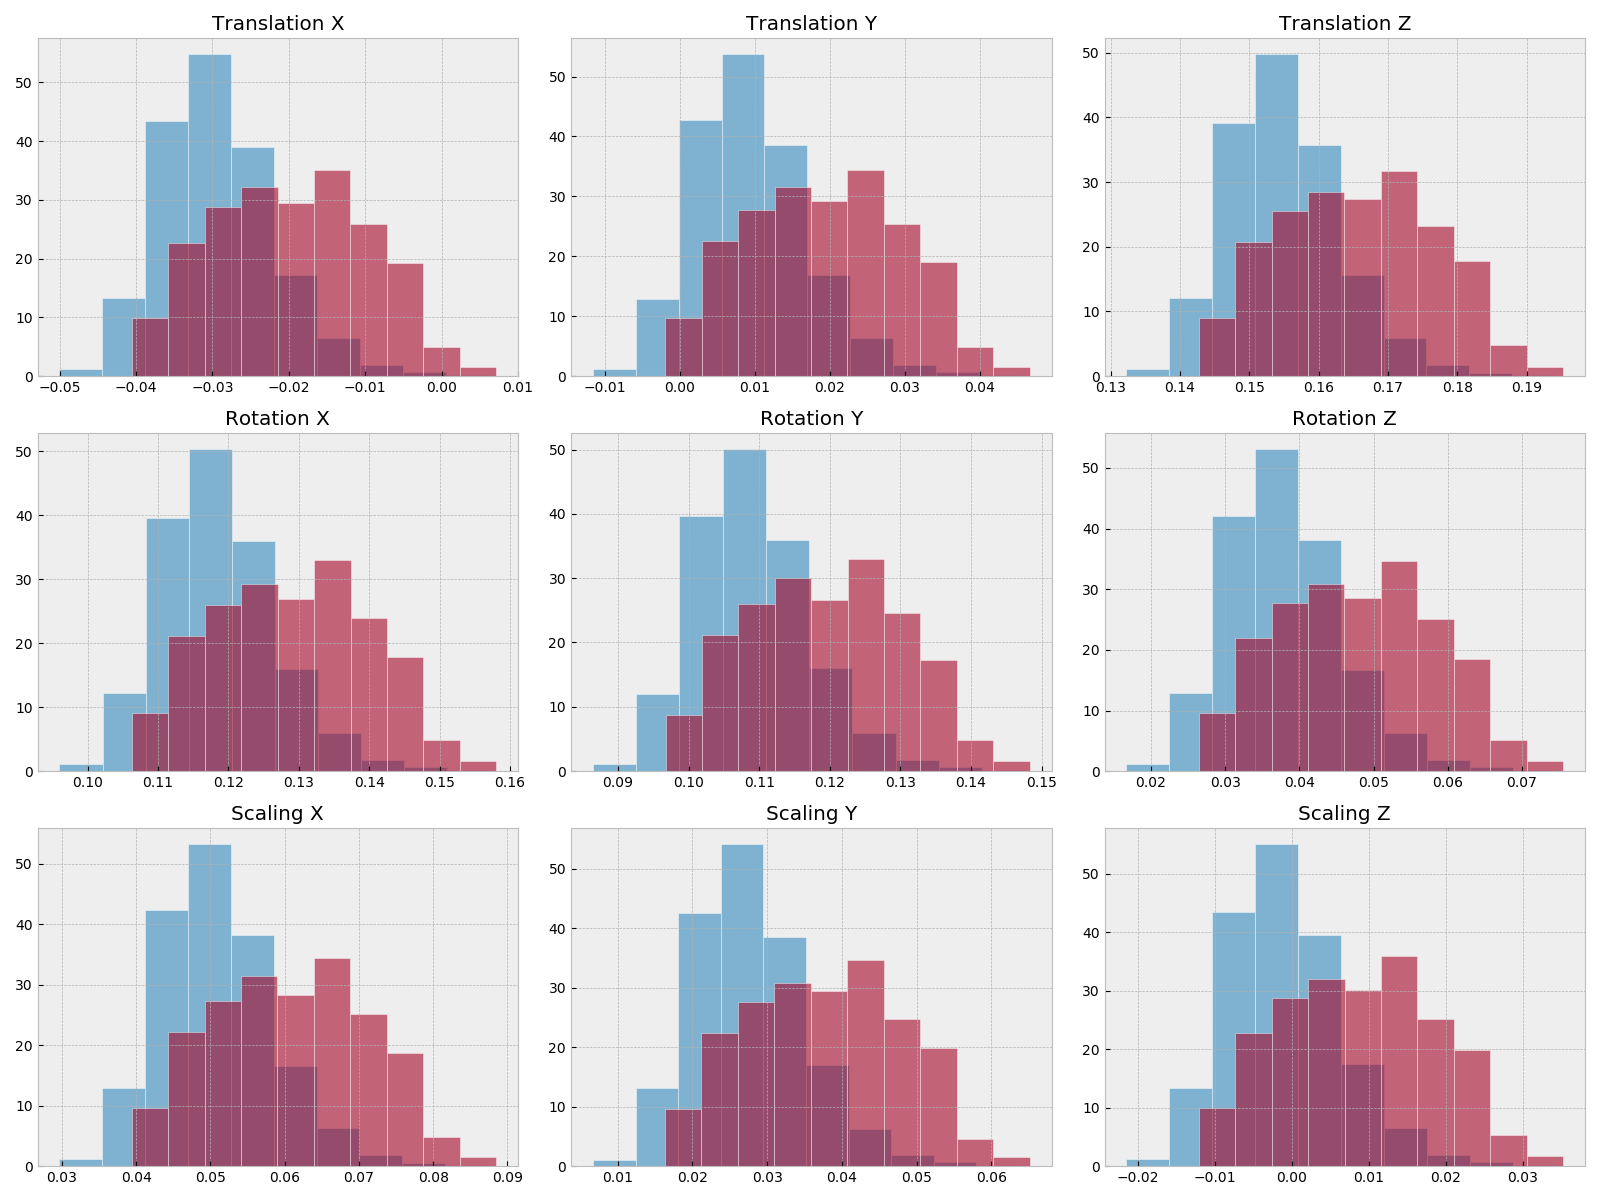
\includegraphics[width=\textwidth]{img_seg/transfo_matrix}
    \caption{Distributions of each parameter of the geometric transformation for the model without penalty. Red is for the adults, blue for the children.}
    \label{fig:transfo_matrix}
\end{figure}

Since the geometric transformation provided an important boost in performance, we look at the distribution of each parameter predicted on the test set in Figure~\ref{fig:transfo_matrix}. 

First we note that the distributions are almost identical for all parameters. Looking at the values for individual images reveals that the parameters are correlated, i.e. if a parameter falls on the lower side of the distribution for an image, the other parameters will also fall on the lower side of their distributions for the same image. This is likely due to using only one convolutional layer to predict the parameters, i.e. a lack of capacity.

The second point of interest is that the distributions between adults and children are very different. The children tends to have lower parameter values and the adults are spread out over a bigger range. This makes sense for the scaling parameters: as the template is based on an adult's kidney, it is necessary to shrink it more to match the size of a children. However there are no reasons why this should be true for the translation and rotation. This is possibly a side-effect of the parameters being so correlated. If the network lacked capacity, it make sense to focus on the most important parameters, the scaling, and the other followed.

Finally, looking at the actual value of the parameters, it seems that the network relies on a very specific transformation to work. Every parameter falls into a narrow range of values. For all images, the template is translated, rotated and scaled in roughly the same direction and amplitude. 

The very low values of the scaling means the template model is heavily shrunk. As a result, the deformation fields must have very high values to match the target. The goal of the $L_2$ penalty is to change this by penalizing high values for the deformation fields.

[TODO why are high values bad ?]

[TODO geometric transfo distributions for penalty model]

%%%%%%%%%%%%%%%%%%%%%%%%%%%%%%%%%%%%%%%%%%%%%%%%%%%%%%%%%%%%%%%%%%%%%%%%%%%%%%%%%%%%%%%%%%%%%%%
\section{Conclusion}

- multiple conv layers for geo pred
